\documentclass[border=0mm]{standalone}
\usepackage{tikz}
\usepackage{amsmath}
\usepackage{amsmath}
\usetikzlibrary{calc, angles, quotes}
\begin{document}
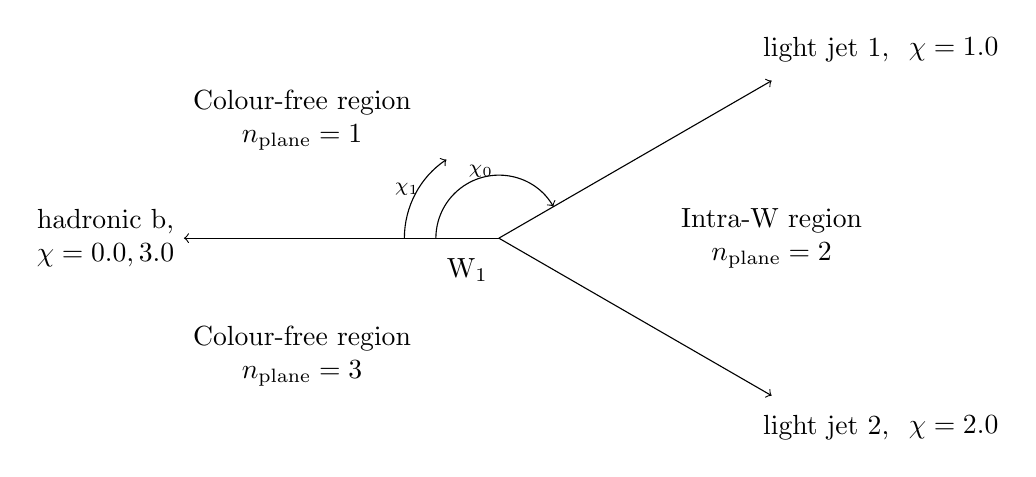
\begin{tikzpicture}
  \newcommand{\ang}{30};
  \coordinate(W1) at (0.0, 0.0);
  \coordinate(c1) at (-4, 0.0);
  \coordinate(c1a) at (-1.0, 1.5);
  \coordinate(c2) at ($({4.0*cos(\ang)}, {4.0*sin(\ang)})$);
  \coordinate(c3) at ($({4.0*cos(30)}, -{4.0*sin(30)})$);
  
  \begin{scope}[local bounding box = inset]
    
    \draw[->] (W1) -- (c1);
    \draw[->] (W1) -- (c2);
    \draw[->] (W1) -- (c3);
    \draw[<-] pic [draw, angle radius=1.2cm, angle eccentricity=1.1,"$\chi_{1}$" font=\scriptsize] {angle=c1a--W1--c1};
    \draw[<-] pic [draw, angle radius=0.8cm, angle eccentricity=1.1,"$\chi_{0}$" font=\scriptsize] {angle=c2--W1--c1};

  \end{scope}
  \node(b1)[align = center] at (inset.east)[anchor=center]{
    Intra-W region\\
    $n_\text{plane}=2$
  };

  \node(b2)[align = center] at (inset.north west)[anchor=center, xshift=1.5cm, yshift=-0.5cm]{
    Colour-free region\\
    $n_\text{plane}=1$
  };

  \node(b3)[align = center] at (inset.south west)[anchor=center, xshift=1.5cm, yshift=0.5cm]{
    Colour-free region\\
    $n_\text{plane}=3$
  };

  \node(t1) at ($(W1)!1.2!(c2)$) {light jet 1,}; \node(t1chi) at (t1.east)[anchor=west]{$\chi=1.0$}; 
  \node(t2) at ($(W1)!1.2!(c3)$) {light jet 2,}; \node(t2chi) at (t2.east)[anchor=west]{$\chi=2.0$};
  \node(t3)[align = center] at (c1)[anchor=east] {hadronic b,\\ $\chi=0.0, 3.0$}; \node(t3chi) at (t3.east)[anchor=west]{};

  \node(l1) at ($(W1) - (0.4, 0.4)$) {$\text{W}_{1}$};

\end{tikzpicture}
\end{document}
